\documentclass{beamer}

% Preamble settings for customization
\usetheme{Madrid} % A popular theme for a clean look
\usecolortheme{dolphin} % A color scheme to pair with the theme
\usepackage{graphicx}
\usepackage{amsmath}
\usepackage{lmodern}
\usepackage{animate}
\usepackage[backend=biber, style=ieee]{biblatex} 
\addbibresource{refs.bib} 
\renewcommand*{\mkbibacro}[1]{#1} % To avoid an error where it was trying to use an unavailable font size in bib

% Presentation metadata
\title{Modeling Global Temperature Variate Effects Over Time}
\author{RJ Cass}
\institute{BYU - Student Research Conference}
\date{28 Feb. 2026}

\begin{document}

% Title slide
\begin{frame}
    \titlepage
\end{frame}

% Table of Contents slide
% \begin{frame}
%     \frametitle{Outline}
%     \tableofcontents
% \end{frame}

% General Notes: More commentary on slides with plots, make it a bit easier to understand if someone zones out, etc. similar to the Week x Latitude (macaroni comment). While presenting, ensure for every plot I explain why I included it, and what we should take out of it

% For EDA plots, include comments on further aggregation (ie. agg over week, or over latitude)

% In plot captions, just put the things I want them to focus on



%%%%%%%%%%%%%%%%%%%%%%%%%%%%%%%%%%%%%%%%%%%%%%%%%%

\section{Introduction}
    %%%%%%%
    \begin{frame}
        \frametitle{Big Picture}
        \begin{itemize}
            \item Attempting to understand the relationship between climate variables (temperature, precipitation) and geography/time
            \begin{itemize}
                \item Want to create a model for Temperature and Precipitation as a function of Latitude, Elevation, and Time
            \end{itemize}
        \end{itemize} 
    \end{frame}

    %%%%%%%
    \begin{frame}
        \frametitle{Motivation}
        \begin{itemize}
            \item Understanding evolution of model parameters in modern climate
            \begin{itemize}
                \item Given a model of climate, how do the coefficients change over time?
            \end{itemize}
            \item Generate general model to apply to ancient data
                \begin{itemize}
                    \item Paleogene era: 66-23 Mya
                    \item Sparse proxy data (fossils, deposition layers, etc.)
                    \item $y(s, t) = x(s, t)^{\top}\beta_t + z(s, t) + \epsilon(s, t)$
                    \item Can learn appropriate structure for design matrix $X$ using modern data
                \end{itemize} 
                % For large portions of the world, the XB portion will be primarily responsible for the modeling, important to get it right
            \item Put me through my paces
        \end{itemize} 
    \end{frame}

    %%%%%%%
    \begin{frame}
        \frametitle{Method}
        ERA5 reanalysis dataset 
            \begin{itemize}
                \item ERA5: 5th generation of ECMWF (European Centre for Medium-Range Weather Forecasts) reanalysis data for last 80 years \cite{CopernicusERA5}
                \item Reanlysis: Uses available data, models, and physical laws to provide a complete and consistent dataset of climate measurements  \cite{CopernicusERA5}
            \end{itemize}

        Data Processing:
        \begin{itemize}
            \item Raw ERA5 data: .25x.25 Latitude grid, daily averages
            \item Aggregated to 1x1 Latitude, weekly averages
            \item Elevation: ERA5 2024 Geopotential, converted to elevation (m)
        \end{itemize} 
    \end{frame}



%%%%%%%%%%%%%%%%%%%%%%%%%%%%%%%%%%%%%%%%%%%%%%%%%%

\section{EDA}
    %%%%%%%
    \begin{frame}
        \frametitle{EDA}

        \begin{figure}[H]
            \centering
            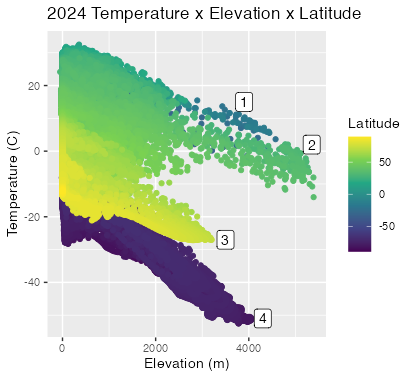
\includegraphics[width=.45\textwidth]{Plots/temp_elev_lat.png}
            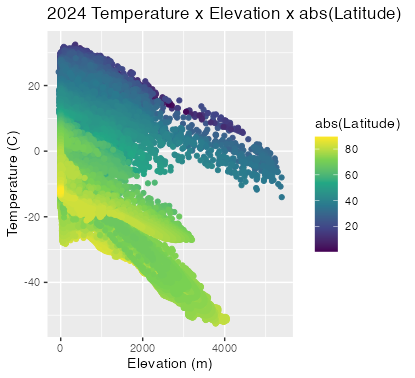
\includegraphics[width=.45\textwidth]{Plots/temp_elev_abs_lat.png}
            \caption{Numbered Regions: 1. Sierras 2. Himalayas 3. Greenland 4. Antarctica. Note the relatively linear effect of elevation, with some irregularities in the poles}
            \label{fig:temp_elev_lat}
        \end{figure}

    \end{frame}

    %%%%%%%
    \begin{frame}
        \frametitle{EDA}

        \begin{figure}[H]
            \centering
            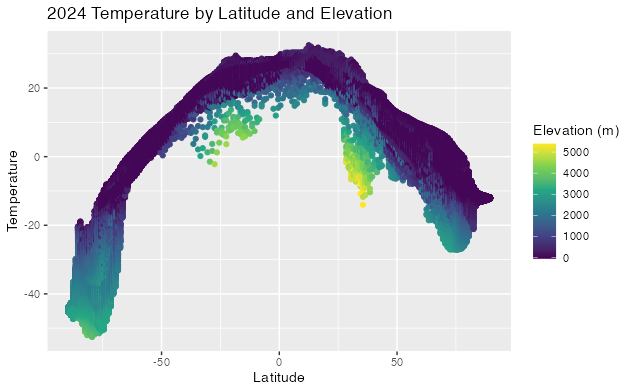
\includegraphics[width=.7\textwidth]{Plots/year_temp_lat_elev.png}
            \caption{Temperatue as a function of Latitude and Elevation interaction. Note the irregular 'rainbow' shape.}
            \label{fig:eda_lat_elev}
        \end{figure}

    \end{frame}

    %%%%%%%
    \begin{frame}
        \frametitle{EDA}

        \begin{figure}[H]
            \centering
            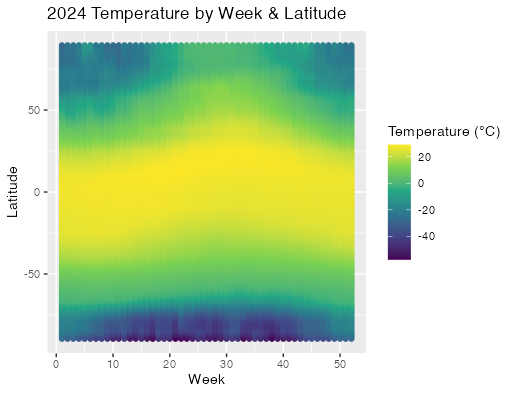
\includegraphics[width=.7\textwidth]{Plots/temp_week_lat.png}
            \caption{Temperature as a function of Week and Latitude. Has a 'macaroni' shape to the middle section, indicating the opposite behavior in the hesmipheres. Has a sharp shift in temperature weeks 17, 45 in the Arctic}
            \label{fig:temp_week_lat}
        \end{figure}

    \end{frame}


    %%%%%%%
    \begin{frame}
        \frametitle{Model Requirements}
        Our model will need to account for the following:
        \begin{itemize}
            \item Interactions between each factor (Week, Latitude, Elevation)
            \item Non-uniform curve by Latitude
            \item Non-uniform curve by Week
                \begin{itemize}
                    \item Particularly opposite North/South Hemsiphere behavior
                \end{itemize}
            \item 'Week' is periodic (need Week$52_{y-1}$ to map into Week$1_y$ smoothly)
            \item Non-centralized peaks in Latitude, Week
        \end{itemize}

    \end{frame}


%%%%%%%%%%%%%%%%%%%%%%%%%%%%%%%%%%%%%%%%%%%%%%%%%%

\section{Results}
    %%%%%%%
    \begin{frame}
        \frametitle{Model}
        \begin{itemize}
        \item $y(s, t) = x(s, t)^{\top}\beta + \epsilon_{s, t}, \epsilon_{s,t} \overset{iid}{\sim} N(0, \sigma^2I)$
        \item Design Matrix given by: $(bs(Lat) + ns(Elev) + bs(Week))^3$
            \begin{itemize}
                \item Includes Latitude, Elevation, Week, all 2 and 3 way interactions
                \item All terms are fit with splines
                \item Boundary conditions enforced on Week: Week 0 = Week 52
            \end{itemize}
        \end{itemize}
    \end{frame}

    %%%%%%%
    \begin{frame}
        \frametitle{Model Comparisons}
        \begin{itemize}
            \item We are considering different models, not a single way to do that
            \item Model Validation/Model Comparison strategies
                \begin{itemize}
                    \item Summary metrics: AIC/BIC, etc. Adding lots of stuff tends to just make it better
                    \item Local Features: look at specific behavior of each model, residuals, etc.
                    \item Want a model that balances the two (ie. really good AIC is not good if it completely ignores a certain region of the earth)
                    \item Paleoclimate data: What level of complexity can that dataset handle? Bias towards simpler model structures
                \end{itemize}
        \end{itemize}
    \end{frame}

    %%%%%%%
    \begin{frame}
        \frametitle{Variable Fits}
        \begin{figure}[H]
            \centering
            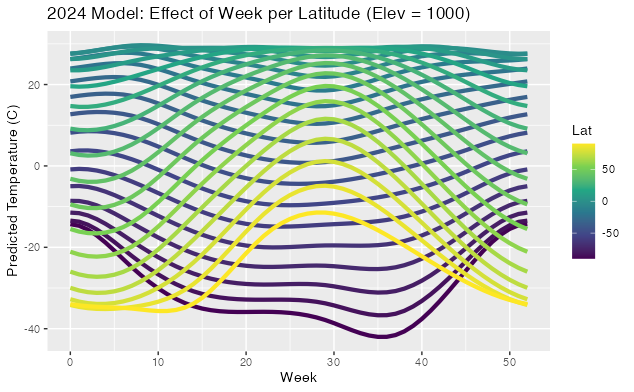
\includegraphics[width=.45\textwidth]{Plots/week_lat_interaction.png}
            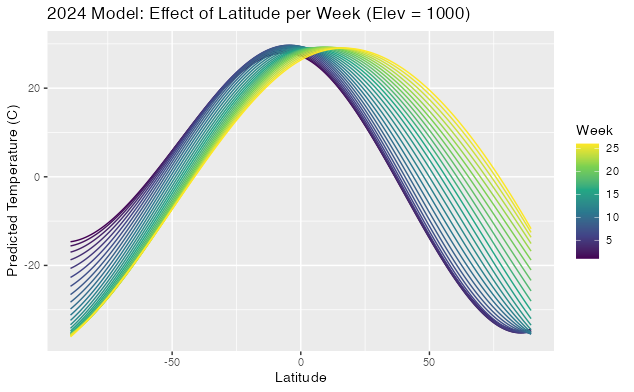
\includegraphics[width=.45\textwidth]{Plots/lat_week_interaction.png}
            \caption{Predicted temperature as s function of Week and Latitude. Note (left) that min/max temperature is offset from middle of year. Also note (right) the steep decline in temperature in high latitudes.}
            \label{fig:var_plots}
        \end{figure}
    \end{frame}

    %%%%%%%
    \begin{frame}
        \frametitle{Residual Analysis}
        \begin{itemize}
            \item Evaluated all residuals across all weeks, found proportion of times the residuals at a location were above a set limit
        \end{itemize}
        
        \begin{figure}[H]
            \centering
            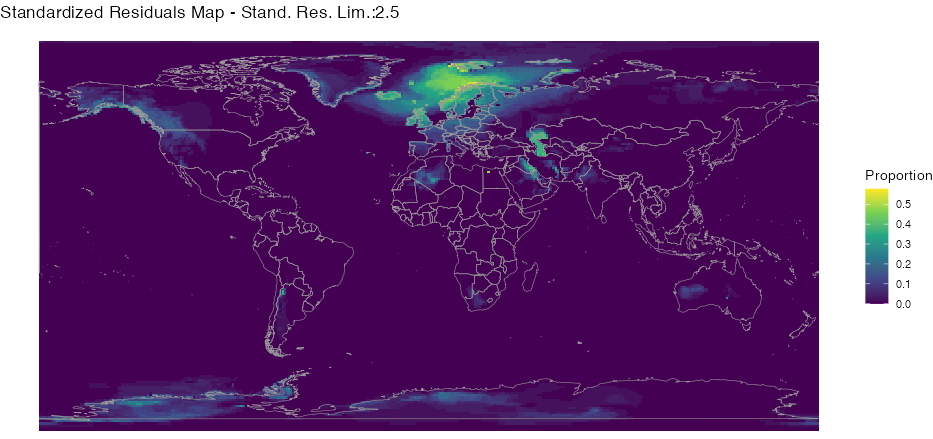
\includegraphics[width = .9\textwidth]{Plots/stand_resid_map_2_5.png} 
            \caption{Proportion per location of residuals over a certain limit. Of interest are the Caspian sea, Norwegian Sea, coastal areas, mountain regions, and some deserts}
            \label{fig:resid_ind_counts}
        \end{figure}
    \end{frame}    


    % \begin{frame}
    %     \frametitle{Geographic Features}
    %         \begin{figure}[H]
    %             \centering
    %             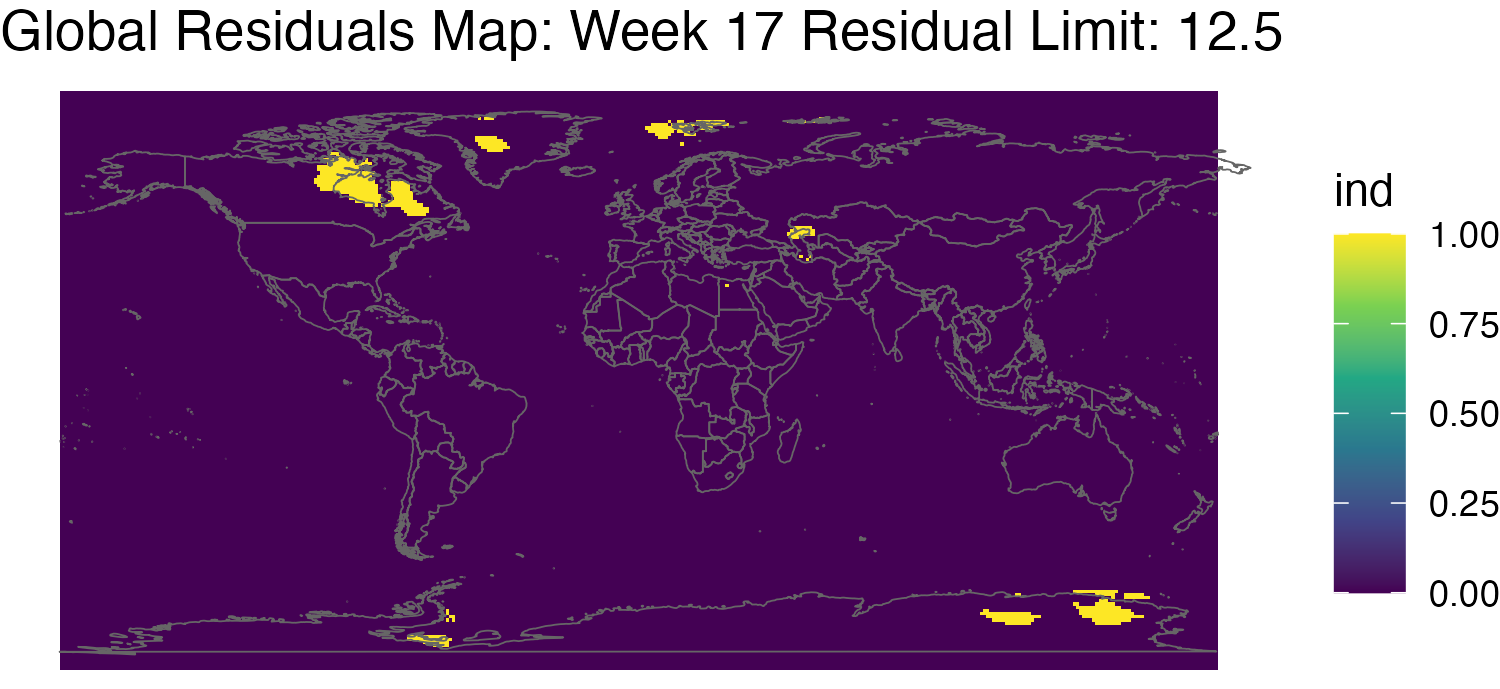
\includegraphics[width = .6\textwidth]{Plots/resid_plot_week_17.png} 
    %             \par
    %             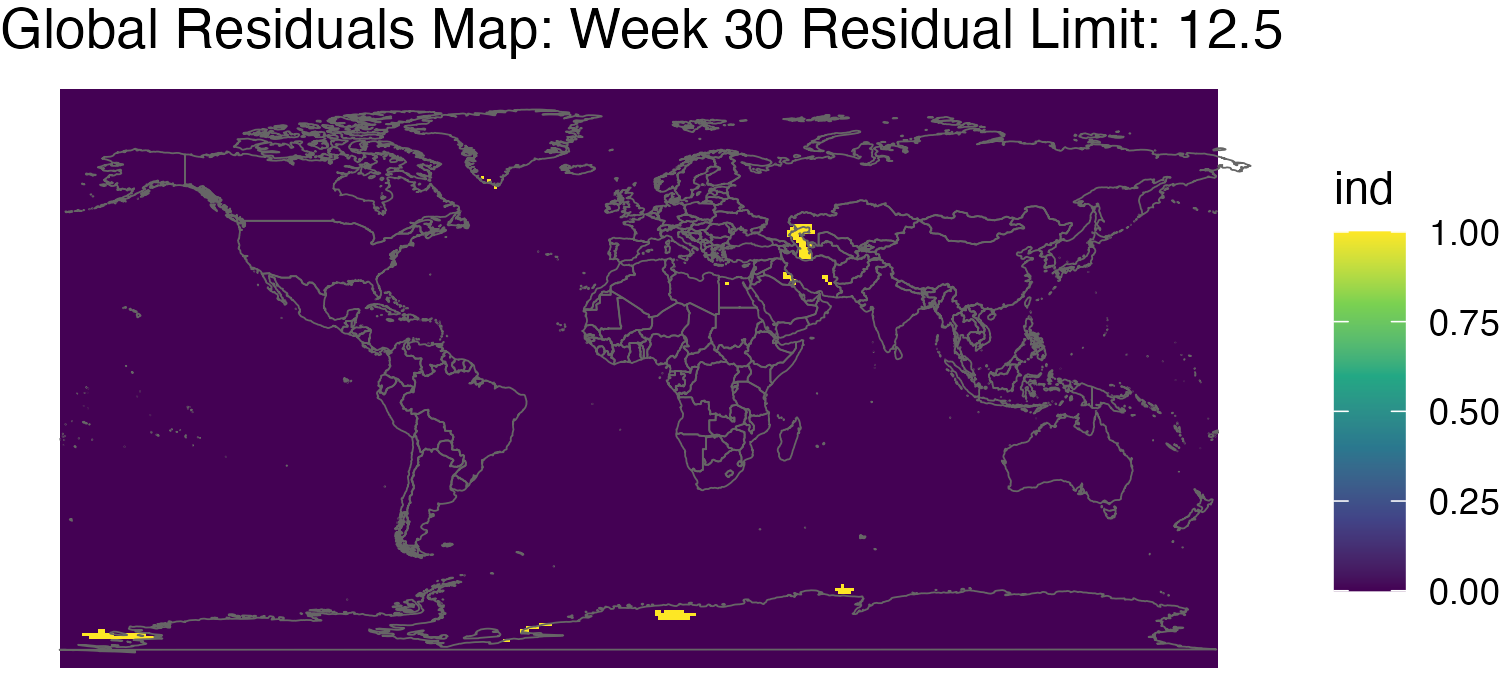
\includegraphics[width=.6\textwidth]{Plots/resid_plot_week_30.png}
    %             \caption{Plots of regions with residuals greater than 12.5. Note large residuals in Hudson Bay, Caspian Sea}
    %             \label{fig:resid_plots}
    %         \end{figure}
    % \end{frame}    

%%%%%%%%%%%%%%%%%%%%%%%%%%%%%%%%%%%%%%%%%%%%%%%%%%

\section{Conclusion}

    %%%%%%%
    \begin{frame}
        \frametitle{Next Steps}
        \begin{itemize}
            \item Additional Data
                \begin{itemize}
                    \item Coast Lines
                    \item Percentage of cell that is water
                    \item Deserts (proxy: NDVI satellite measure of vegetation) 
                \end{itemize}
            \item Model Improvements
                \begin{itemize}
                    % \item Revisit Elevation 
                    \item Explore models, pick a final candidate 
                    \item Account for spacial and temporal correlation
                    \begin{itemize}
                        \item Massive dataset, look into Vecchia
                    \end{itemize}
                \end{itemize}
            \item Further Analyses
                \begin{itemize}
                    \item Fit model to previous years, see how coefficients change
                    \item Apply similar techniques to Precipitation
                \end{itemize}
        \end{itemize}

    \end{frame}   

    \begin{frame}
        \frametitle{Conclusion}
            \begin{itemize}
                \item Obtained and aggregated ERA5 
                \item Created model of temperature using Latitude, Elevation, Week
                \item Investigated residuals of model to identify features that still need to be addressed
                \item Future work will focus on collecting new data features, making improvements to model, and applying model to new years/climate variables
            \end{itemize}
    \end{frame}   


\section{Appendix}
    \begin{frame}{Bibliography}
        \frametitle{Bibliography}

        \printbibliography

    \end{frame}

\end{document}